\documentclass{article}
\usepackage{tikz}
\usetikzlibrary{shapes.geometric, arrows.meta, positioning, calc, shadows}
\usepackage{amsmath}
\usepackage{ragged2e}
\usepackage{xcolor}
\usepackage{enumitem}
\usepackage[margin=0.5in]{geometry}

\begin{document}

\begin{figure}[!h]
\centering
\resizebox{\textwidth}{!}{%
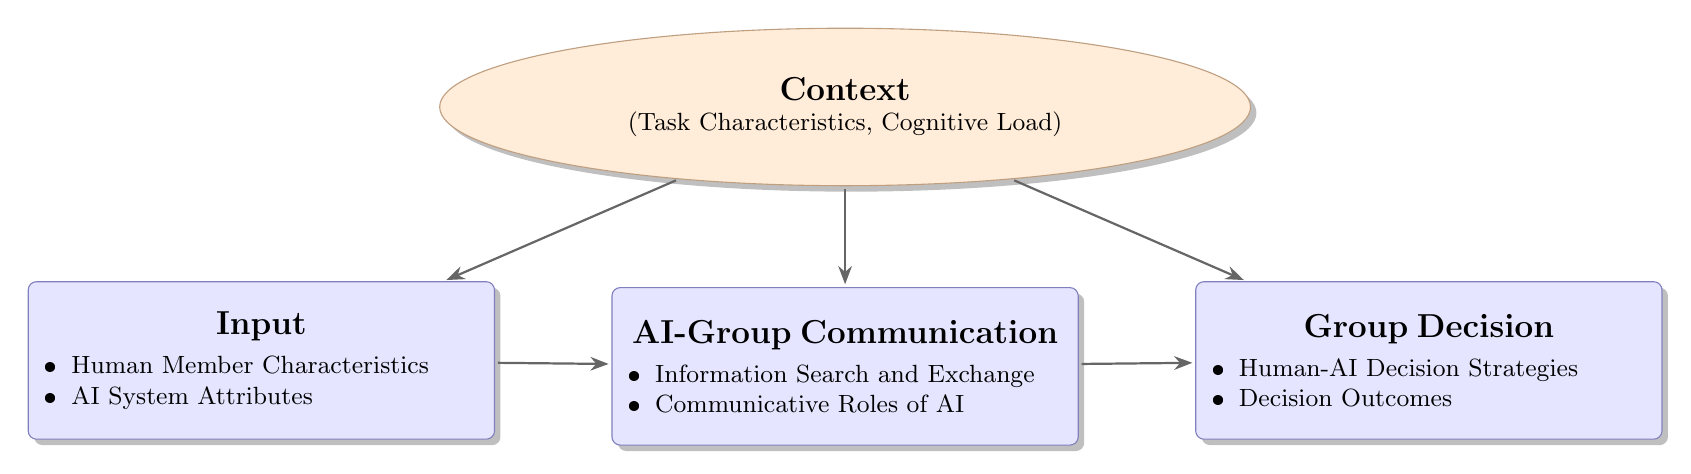
\begin{tikzpicture}[
    node distance=1.5cm and 0.8cm,
    >=Stealth,
    auto,
    box/.style={
        draw,
        rectangle,
        align=center,
        minimum height=2.0cm,
        text width=5.5cm,
        inner sep=6pt,
        font=\small,
        fill=blue!10,
        draw=blue!50!black!50,
        rounded corners=3pt,
        drop shadow={fill=black!50, shadow xshift=0.5ex, shadow yshift=-0.5ex}
    },
    ellipse_style/.style={
        draw,
        ellipse,
        align=center,
        minimum height=2.0cm,
        text width=7.0cm,
        inner sep=4pt,
        font=\small,
        fill=orange!15,
        draw=orange!50!black!50,
        drop shadow={fill=black!50, shadow xshift=0.5ex, shadow yshift=-0.5ex}
    },
    arrow/.style={
        ->,
        shorten >=1pt,
        shorten <=1pt,
        line width=0.8pt,
        draw=gray!80!black,
    }
]

% -- Context at the Top --
\node[ellipse_style] (context) {\textbf{\large Context} \\ (Task Characteristics, Cognitive Load)};

% -- Three Main Boxes Below --
\node[box, below left=of context] (input) {\textbf{\large Input}
    \begin{itemize}[leftmargin=*, itemsep=0pt, parsep=0pt, topsep=3pt]
        \item Human Member Characteristics
        \item AI System Attributes
    \end{itemize}
};

\node[box, below=of context, yshift=0.22cm] (ai_comm) {\textbf{\large AI-Group Communication}
    \begin{itemize}[leftmargin=*, itemsep=0pt, parsep=0pt, topsep=3pt]
        \item Information Search and Exchange
        \item Communicative Roles of AI
    \end{itemize}
};

\node[box, below right=of context] (group_decision) {\textbf{\large Group Decision}
    \begin{itemize}[leftmargin=*, itemsep=0pt, parsep=0pt, topsep=3pt]
        \item Human-AI Decision Strategies
        \item Decision Outcomes
    \end{itemize}
};

% -- Arrows --
\draw[arrow] (context) -- (input);
\draw[arrow] (context) -- (ai_comm);
\draw[arrow] (context) -- (group_decision);
\draw[arrow] (input) -- (ai_comm);
\draw[arrow] (ai_comm) -- (group_decision);

\end{tikzpicture}
}%
\caption{An Information-Processing Framework for Human-AI Decision Making in Groups}
\label{fig:framework}
\end{figure}

\end{document}
